\documentclass[
%draft%     uncomment to activate draft mode (see preamble/proofs)
]{article}   

% preamble -- do not rearrange order of \includes
%\include{classoptions}
%\include{pagesize}
%\include{packages}
%\include{encoding}         
%\include{fonts}
%\include{ToC}
%\include{contributor}
%\include{copyright}
%\include{bibtex}
%\include{environments}
%\include{sectionoptions}
%\include{headerfooter}
%\include{footnoteformat}
%\include{codesnipets}
%\include{proofs}

\usepackage{tikz}
\usepackage{graphicx}
\usepackage[export]{adjustbox}
\usepackage{caption}
\usepackage{amssymb}
\usepackage{float}
%\usepackage{minted}
\usetikzlibrary{shapes}
\usetikzlibrary {positioning}

\usepackage{geometry}
\usepackage{array}
\usepackage{hyperref}
\hypersetup{
    colorlinks=true,
    linkcolor=magenta,
    filecolor=cyan,      
    urlcolor=blue,
}
\graphicspath{ {./images/} }

% define issue details
\title{Compiler Optimization Notes}
\newcommand\thejournalsubtitle{Notes compiled for the Compiler Optimization Course}
\newcommand\thevolume{}
\newcommand\theseason{February}
\newcommand\theyear{2021}
\newcommand\theissue{\thejournal \ \thevolume \ (\theyear)} 
\newcommand\generaleditor{}
\newcommand\associateeditor{}
\sloppy
\newcommand\thewebsite{https://iitd.github.io/col729}

\begin{document}
\sloppy                         % preferences more space between words over overrunning margins
\lefthyphenmin=3                % suppresses hyphenation after only 1 or 2 characters
                                % NB: You will need to repeat \lefthyphenmin in the text if you use \selectlanguage
%\include{editorialboard}
%\include{titlepage}
%\include{colofon}
\pagenumbering{roman}           
%\tableofcontents  
\thispagestyle{empty}

% \include{essays/preface}
\pagenumbering{arabic}
%\part{COL729 Lecture Modules and Discussions}
\input{../module68}
\input{../module69} 
\input{../module70}
\input{../module71} 
\input{../module72}
\input{../module73} 
\input{../module74}
\input{../module75} 
\input{../module76}
\input{../module77} 
\input{../module78} 
\input{../module79}
\input{../module80}
\input{../feb19discussion}
\input{../module81} 
\input{../module82}
\input{../module83} 
\input{../module84}
\input{../feb26discussion}
\input{../module85} 
\input{../module86}
\input{../module87} 
\input{../module88}
\input{../module89}
\input{../module90}
\input{../module91} 
\input{../module92}
\input{../module93} 
\input{../module94}
\input{../module95} 
\input{../module96}
\input{../module97} 
\input{../module98}
\section {Family of Transfer Functions}
\setlength{\parindent}{0pt}
(Prepared by Sanket Gandhi)

\vspace{0.3cm}
\begin{itemize}
    \item Recall that a DFA is defined by ($F$, $V$, \^{}) where ($V$, \^{}) forms the semilattice and $F$ is family of transfer functions.
    \item Family of Transfer Functions $F$ is set of functions. For particular DFA each transfer function for an instruction or a basic block is drawn from the set $F$. 
    \item If transfer function does not have certain properties then DFA may not terminate. $F$ should have certain properties in order to reason about optimality and convergence of DFA.
\end{itemize}

\subsection{Properties of Family Transfer Functions F}
Family of transfer functions $F$ must have following properties.  
\begin{itemize}
    \item Every function is $F$ takes a value from DFA value set $V$ and returns a value from same set $V$, that is every function $f$ in $F$ have form $f:V \rightarrow V $
    \item F contains the identity function that is, $\exists \ f \in F \ $ such that $f(x) = x $, $ \forall \ x \in V$. \\ This property is needed because in case of NOP instructions the output is equal to input. So identity function should be in $F$.  
    \item F is closed under composition, if $f_{1},f_{2} \in F$ then $f_{1}\circ f_{2} \in F$.\\ This property will be helpful for defining transfer functions for basic blocks.
\end{itemize}

\subsection{Example}
Many of the DFAs(Reaching definitions, Constant Propagation etc.) have following structure in transfer function.
\[f(x) = (x-kill_{s})\bigcup gen_{s}\] for some instruction $s$. $kill_{s}$ and $gen_{s}$ only depends on $s$ and are independent of $x$.
\\$F$ is the set of function which is populated by changing $kill$ and $gen$ set in above structure.
In case of reaching definitions if we have $n$ definitions in program then size of $F$ will be $4^{n}$.  Lets check whether $F$ is family of transfer functions or not.
\begin{itemize}
    \item Every function in $F$ take a set of some kind $x$ input and perform set operations. The output is also set of same kind. $F$ have first property of family of transfer function.
    \item In case of $gen = \emptyset$ and $kill = \emptyset$, the transfer function will become $f(x) = x$ and $f\in F$.
    \item Consider two functions $f_{1}(x) = (x-kill_{1})\bigcup gen_{1}$ and $f_{2}(x) = (x-kill_{2})\bigcup gen_{2}$. Both $f_{1}, f_{2}$ belongs to $F$. 
    \[f_{2}(f_{1}(x)) = ((x-kill_{1})\bigcup gen_{1}-kill_{2})\bigcup gen_{2}\]
    By using property $A\bigcup B - C = (A-C)\bigcup (B-C)$ the above equation becomes
    \[f_{2}(f_{1}(x)) = (x-(kill_{1} \bigcup kill_{2}))\bigcup ((gen_{1}-kill_{2})\bigcup gen_{2})\]
    With $kill_{1\circ 2} = kill_{1} \bigcup kill_{2}$ and $gen_{1\circ 2} = (gen_{1}-kill_{2})\bigcup gen_{2}$ the composite function becomes $f_{2}(f_{1}(x)) = (x - kill_{1 \circ 2})\bigcup gen_{1\circ 2}$. Therefore $f_{1} \circ f_{2} \in F$ as $F$ contain transfer functions with all possible $gen$ and $kill$ set. 
\end{itemize}
 
\section {Monotonicity of DFA Framework}
\setlength{\parindent}{0pt}
(Prepared by Sanket Gandhi)

\vspace{0.3cm}
\begin{itemize}
    \item Recall that we require semilatiice ($V$,\^{}) to have finite height with some properties over $F$ to guarantee convergence property of the fixed point  iteration.
    \item Also recall that family of transfer function have three properties, all functions in $F$ should be of form $V$ to $V$, $F$ should contain identity function and $F$ should be closed under composition. Do we have additional requirements from $F$ to guarantee convergence of fixed point iteration?
\end{itemize}

\subsection{Example}
Consider DFA ($F$,$V$,\^{})* with $V = \{true, false\}$, \^{}$= logical \ and $, $F = \{id,not,True,False\}$. The transfer functions are defined as follows:
\[id(x) = x, \ \ \forall x \in V \]
\[not(true) = false\]
\[not(false) = true\]
\[True(x) = true, \ \ \forall x \in V \]
\[False(x) = true, \ \ \forall x \in V \]
\begin{figure}[h!]
\caption{Semilattice diagram of *}
\begin{center}
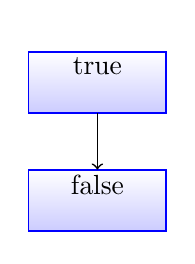
\begin{tikzpicture}[-latex ,auto ,node distance =1.5cm and 2cm ,on grid ,
    semithick ,
    state/.style ={ rectangle ,top color =white , bottom color = blue!20 ,
    draw, blue , text=blue , scale = 0.7 ,minimum width =2.5 cm, minimum height = 1.1 cm}]
    \node[state] (A){} node [label = {}, rectangle split,rectangle split parts=2]{%
      true%
      };
    \node[state] (E) [below =of A]{} node [label = {},rectangle split,rectangle split parts=2] [below = of A] {%
      false%
      };
    \path[->] (A) edge node [above = 0.2 cm] {} (E);
    
\end{tikzpicture}
\end{center}
\label{fig:semilattice_and}
\end{figure}
\begin{itemize}
    \item Note that semilattice have finite height 2.
    \item Every function in $F$ is of form $V \rightarrow V$
    \item $F$ contains the identity function which is $id$.
    \item $F$ is closed under composition
\end{itemize}
The $F$ is valid family of transfer functions. Consider following instance of program. Basic block $B1$ have transfer function $id$ and basic block $B2$ have $not$ transfer function. By boundary condition and initialization of intermediate program point with top value the initial state is also shown in following figure. 
\begin{figure}[ht]
    \centering
    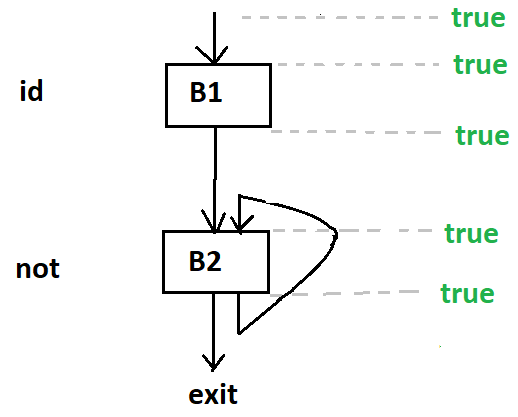
\includegraphics[scale= 0.4]{images/100-1.png}
    \caption{Initial State}
\end{figure}
When iterative fixed point algorithm first time reaches basic block $B2$ it meets over incoming  edges which is logical and of $true$. The out value of $B2$ and hence one of the in edge value of $B2$ become $not(true)$ which is $false$. The meet operator is logical and so the in value of $B2$ also becomes false.
\begin{figure}
    \centering
    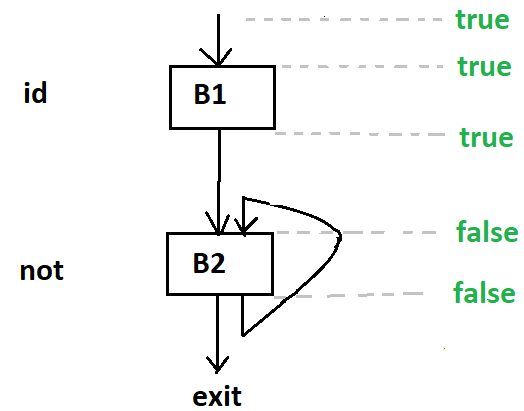
\includegraphics[scale= 0.4]{images/100-2.png}
    \caption{After FPI reaches B2 first time}
\end{figure}
As the $in[B2]$ and $out[B2]$ are not satisfying the transfer function condition FPI will again reach to $B2$. The $in[B2]$ and $out[B2]$ will again become $true$. Even our DFA framework follows all properties discussed earlier the algorithm will never converge. 
\begin{itemize}
    \item There should be some more constraints on family of transfer function $F$ so to guarantee convergence of FPI.  
    \item The problem is $not$ function in $F$ which keeps oscillating between two values. It is expected that the transfer function should keep same order in output values as that of input values(if it is defined).  
\end{itemize}
\subsection{Monotonicity of DFA framework}
A DFA framework ($F$,$V$,\^{}) is monotone if and only if
\[if \ \ \ \ x \leq y \ \ \ implies \ \ \ f(x) \leq f(y) \ \ \ \forall f \in F \ \ \ \ \forall x,y \in V\]
\begin{itemize}
    \item This says that if DFA framework is monotone then for all transfer functions in $F$ if there is particular order in input values then corresponding output values will also follow same order.
    \item In above examples $true \geq false$ but $not(true) \ngeq not(false)$, hence above DFA framework was not monotone.
    \item Equivalently a framework is monotone if and only if $f(x$\^{}$y) \leq f(x)$\^{}$f(y)$.
    The proof for DFA monotonicity implies $f(x$\^{}$y) \leq f(x)$\^{}$f(y)$ was provided in live session and is as follows:\\
    \textit{Proof:} By definition of meet operator,
    $a$\^{}$b \leq a$ and  $a$\^{}$b \leq b$. As DFA framework is monotone for all tansfer functions $f(a$\^{}$b) \leq f(a)$ and $f(a$\^{}$b) \leq f(b)$ holds. Now $f(a$\^{}$b) \leq f(b)$ implies $f(a$\^{}$b)$\^{}$f(b) = f(a$\^{}$b)$. Similarly $f(a$\^{}$b) \leq f(a)$ implies $f(a$\^{}$b)$\^{}$f(a) = f(a$\^{}$b)$. Now consider $(f(a)$\^{}$f(b))$\^{}$f(a$\^{}$b)$ is same as as $(f(a)$\^{}$f(b))$\^{}$(f(a$\^{}$b)$\^{}$f(a$\^{}$b))$. By using properties of meet operator the above expression is same as 
    $(f(a)$\^{}$f(a$\^{}$b))$\^{}$(f(b)$\^{}$f(a$\^{}$b))$. Which further boils down to $f(a$\^{}$b)$\^{}$f(a$\^{}$b)$ = $f(a$\^{}$b)$. At the end $(f(a)$\^{}$f(b))$\^{}$f(a$\^{}$b)$ = $f(a$\^{}$b)$. Therefore $f(a)$\^{}$f(b) \geq f(a$\^{}$b)$.
    \item Also in example discussed above $not(false$\^{}$true) = true$ and $not(true)$\^{}$not(false)=false$. Which means $not(false$\^{}$true) \nleq not(false)$\^{}$not(true)$ and so DFA framework in example was not monotone.

\subsection{Monotone DFA Example}
Consider the reaching definitions DFA ($F$,$V$,\^{}). The transfer function in this framework is of type $f(x) = (x-kill)\bigcup gen$. The values in this framework are set of definitions. If $x\leq y$ then this implies $x \supseteq y$ for $x,y \in V$. For transfer function $f\in F$ and $x_{1},x_{2} \in V$,
\[f(x_{1}) = (x_{1}-kill)\bigcup gen\]
\[f(x_{2}) = (x_{2}-kill)\bigcup gen\]
Clearly if $x_{1} \leq x_{2}$ implies $x_{1} \supseteq x_{2}$ which implies $f(x_{1}) \supseteq f(x_{2})$. This implies $f(x_{1}) \leq f(x_{2})$. This shows ($F$,$V$,\^{}) is monotone. 
\end{itemize}
%\include{../module101} 
%\include{../module102}
%\include{../module103} 
%\include{../module104}
%\include{../module105} 
%\include{../module106}
%\include{../module107} 
%\include{../module108}
%\include{../module109} 
%\include{../module110}
%\include{../module111} 
%\include{../module112}
%\include{../module113} 
%\include{../module114}
%\include{../module115} 
%\include{../module116}
%\include{../module117} 
%\include{../module118}
%\include{../module119} 
%\include{../module120}
%\include{../module121} 
%\include{../module122}
%\include{../module123} 
%\include{../module124}
%\include{../module125} 
%\include{../module126}
%\include{../module127} 
%\include{../module128}
%\include{../module129} 
%\include{../module130}
%\include{../module131} 
%\include{../module132}
%\include{../module133} 
%\include{../module134}
%\include{../module135} 
%\include{../module136}
%\include{../module137} 
%\include{../module138}
%\include{../module139} 
%\include{../module140}
%\include{../module141} 
%\include{../module142}
%\include{../module143} 
%\include{../module144}
%\include{../module145} 
%\include{../module146}
%\include{../module147} 
%\include{../module148}
%\include{../module149} 
%\include{../module150}
\end{document}
